% Created 2019-11-21 Thu 10:45
% Intended LaTeX compiler: pdflatex
\documentclass[compress,presentation,aspectratio=169]{beamer}
\usepackage[utf8]{inputenc}
\usepackage[T1]{fontenc}
\usepackage{fontspec}
\setmonofont{DejaVu Sans Mono}
\usepackage{graphicx}
\usepackage{grffile}
\usepackage{longtable}
\usepackage{wrapfig}
\usepackage{rotating}
\usepackage[normalem]{ulem}
\usepackage{amsmath}
\usepackage{textcomp}
\usepackage{amssymb}
\usepackage{capt-of}
\usepackage{hyperref}
\usepackage{minted}
\usetheme{default}
\author{Mauro Werder}
\date{\today}
\title{Introducing Julia: A fast \& fun dynamic programming language}
\hypersetup{
 pdfauthor={Mauro Werder},
 pdftitle={Introducing Julia: A fast \& fun dynamic programming language},
 pdfkeywords={},
 pdfsubject={},
 pdfcreator={Emacs 26.3 (Org mode 9.1.9)},
 pdflang={English}}
\begin{document}


\begin{frame}[fragile,label={sec:org6062e64}]{}
\frametitle{\LARGE Julia: A fast \& fun dynamic programming language}
\begin{center}

\includegraphics[width=.2\linewidth]{./figs/julia-logo.png}\quad 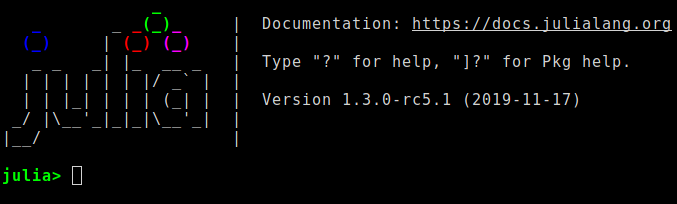
\includegraphics[width=.3\linewidth]{./figs/julia-repl.png}
\end{center}
\vspace{2cm}
by Mauro Werder (github: @mauro3, werder@vaw.baug.ethz.ch)


\end{frame}

\begin{frame}[fragile,label={sec:org6062e64}]{}
\frametitle{Who am I?}
\begin{itemize}
\item Oberassistent in the glaciology group of Daniel Farinotti @ WSL and ETHZ
\begin{itemize}
\item besides numerical work I also do field and lab experiments
\end{itemize}
\pause
\item Julia user \& contributor since 2013
--> probably one of the earliest adopters in Switzerland
    (Julia was first released in 2012)
\begin{itemize}
\item maintainer of five Julia packages:
\begin{itemize}
\item \href{https://github.com/mauro3/Parameters.jl}{Parameters.jl} -- easier handling of large structs of parameters
\item \href{https://github.com/mauro3/UnPack.jl}{UnPack.jl} -- packing and unpacking of data-structures
\item \href{https://github.com/mauro3/SimpleTraits.jl}{SimpleTraits.jl} -- a simple trait system
\item \href{https://github.com/mauro3/WhereTheWaterFlows.jl}{WhereTheWaterFlows.jl} -- a water-routing code
\item \href{https://github.com/mauro3/KissMCMC.jl}{KissMCMC.jl} -- a Markov chain Monte Carlo sample
\end{itemize}
\end{itemize}
\item besides my research I use Julia in teaching at ETHZ:
  \begin{itemize}
  \item Physics of Glaciers
  \item Solving PDEs in parallel on GPUs with Julia
    \url{https://eth-vaw-glaciology.github.io/course-101-0250-00/}
  \end{itemize}
\end{itemize}
\end{frame}


\begin{frame}[fragile,label={sec:org6062e64}]{What does Julia code
    look like?}
  \footnotesize
 \begin{block}{Example, solve Lorenz system of ODEs:}
\begin{minted}[mathescape=true,linenos=false,numbersep=5pt,frame=lines,framesep=2mm]{julia}
using OrdinaryDiffEq, Plots

function lorenz(x, p, t)
    σ = 10
    β = 8/3
    ρ = 28
    return [σ*(x[2]-x[1]), x[1]*(ρ-x[3]), x[1]*x[2] - β*x[3]]
end

# integrate dx/dt = lorenz(t,x) numerically from t=0 to t=50
# and IC x₀
tspan = (0.0, 50.0)
x₀ = [2.0, 0.0, 0.0]
sol = solve(ODEProblem(lorenz, x₀, tspan), Tsit5())

plot(sol, vars=(1,2,3)) # plot Lorenz attractor
\end{minted}
\end{block}
\end{frame}

\begin{frame}[fragile,label={sec:org613e3fa}]{What does Julia code
    look like?}
    \footnotesize
 \begin{minted}[mathescape=true,linenos=false,numbersep=5pt,frame=lines,framesep=2mm]{julia}
plot(sol, vars=(1,2,3)) # plot Lorenz attractor
\end{minted}

\begin{center}
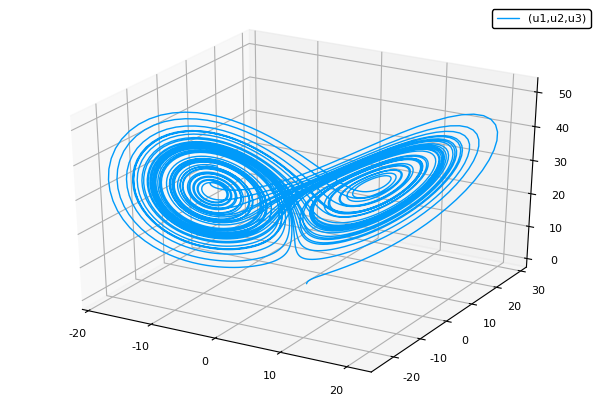
\includegraphics[width=.6\linewidth]{./figs/lorenz.png}
\end{center}
\end{frame}

\begin{frame}[label={sec:orgf4971a5}]{Julia in brief}
      \footnotesize
\begin{block}{Julia 1.0 was released in 2018, current version is 1.8}
\end{block}

\begin{block}{Features}
\begin{itemize}
\item general purpose language with a focus on technical computing
\item dynamic language
\begin{itemize}
\item interactive development
\item garbage collection: no manual memory management
\end{itemize}
\item good performance on par with C \& Fortran (through just-ahead-of-time compilation)
\begin{itemize}
\item No need to vectorize: for-loops are fast
\end{itemize}
\item multiple dispatch
\item user-defined types are as fast and compact as built-ins
\item Lisp-like macros and other metaprogramming facilities
\item designed for parallelism and distributed computation
\item good inter-op with other languages
\end{itemize}
\end{block}
\end{frame}

\begin{frame}[label={sec:org28a3717}]{Ok, but why?}
  \footnotesize
\alert{The two language problem}

\begin{block}{One language to prototype   ---  one language for production}
\begin{itemize}
\item example my institute: GREMS re-write from IDL to C(++)
\end{itemize}
\end{block}

\begin{block}{One language for the users  ---  one language for under-the-hood}
\begin{itemize}
\item Numpy (python --- C)
\item machine-learning: pytorch, tensorflow
\end{itemize}
\end{block}
\end{frame}

\begin{frame}[label={sec:orgeb77589}]{Ok, but why?}
  \footnotesize
\alert{The two language problem}

\begin{block}{One language to prototype   ---  one language for production}
\begin{itemize}
\item example my institute: GREMS re-write from IDL to C(++)
\end{itemize}
\end{block}

\begin{block}{One language for the users  ---  one language for under-the-hood}
\begin{itemize}
\item Numpy
\item machine-learning: pytorch, tensorflow
\end{itemize}

\begin{center}
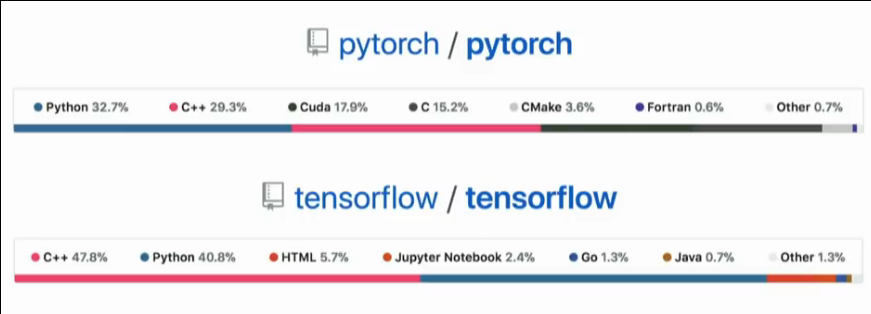
\includegraphics[width=.7\linewidth]{./figs/ml.png}
\end{center}
\end{block}
\end{frame}

\begin{frame}[label={sec:orgb7aee9c}]{Two language problem}
  \footnotesize
Prototype/interface language:
\begin{itemize}
\item easy to learn and use
\item interactive
\item productive
\item --> \alert{but slow}
\item Examples: Python, Matlab, R, IDL\ldots{}
\end{itemize}

Production/fast language:
\begin{itemize}
\item fast
\item --> \alert{but} complicated/verbose/not-interactive/etc
\item Examples: C, C++, Fortran, Java\ldots{}
\end{itemize}
\end{frame}

\begin{frame}[label={sec:orgda7d66a}]{Julia solves the two-language problem}
  \footnotesize
Julia is:
\begin{itemize}
\item easy to learn and use
\item interactive
\item productive
\end{itemize}

and also:
\begin{itemize}
\item fast
\end{itemize}

\alert{This blurs the line between users and developers!}
\end{frame}

\begin{frame}[label={sec:org4c6a2e0}]{Julia solves the two-language problem}
  \footnotesize
Example:

\begin{center}
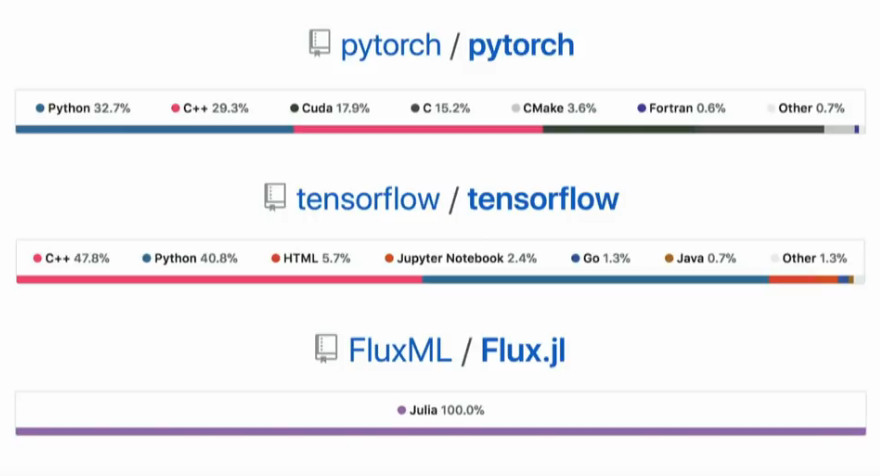
\includegraphics[width=.7\linewidth]{./figs/flux-vs-tensorflow.png}
\end{center}

Flux is a pure Julia deep learning package.   This is possible, because Julia runs at native speed
both on the CPU and GPU.
\end{frame}

\begin{frame}[fragile,label={sec:org8723e64}]{The good: easy to learn}
  \footnotesize
 \begin{itemize}
\item the basics of Julia are as simple to learn as Python, Matlab, etc

\item however, the language has many powerful/advanced features which can
be accessed as the programmer progresses in skills (rich type
system, multiple dispatch, meta-programming, access to compiler)
--> \alert{the language grows with the user}

\item writing code is very close to mathematics (not like the Python/Numpy
stuff)
--> one reason this works so well is \emph{multiple dispatch} (next slide)
\end{itemize}
\end{frame}

\begin{frame}[fragile,label={sec:org8723e64}]{The good: nice syntax,
    cool features}
  \footnotesize
Examples:\\[2mm]

Compact function definition and unicode:
\begin{minted}[mathescape=true,linenos=false,numbersep=5pt,frame=lines,framesep=2mm]{julia}
ϕ(t) = sin(2π * t)\\[1mm]
\end{minted}

\pause
Vectorized function application:
\begin{minted}[mathescape=true,linenos=false,numbersep=5pt,frame=lines,framesep=2mm]{julia}
ϕ.([1,2,3]) .+ [4,5,6]
\end{minted}
(note, this gets fused into one loop, no temporary arrays are created)\\[1mm]
\pause

Parametric types
\begin{minted}[mathescape=true,linenos=false,numbersep=5pt,frame=lines,framesep=2mm]{julia}
struct Point{N, T}
    coords::NTuple{N,T}
end
Point((3,4))   # 2D -> Point{2, Int64}((3, 4))
Point((3,4,5)) # 3D -> Point{3, Float64}((3.0, 4.0, 5.0))
\end{minted}


\end{frame}

\begin{frame}[label={sec:org1e274f0}]{Interlude: multiple dispatch}
  \footnotesize
\begin{itemize}
\item Julia is \textbf{not} an object oriented language
\end{itemize}

Object oriented:
\begin{itemize}
\item methods belong to objects
\item method is selected based on first argument (self)
\end{itemize}

Multiple dispatch:
\begin{itemize}
\item methods are separate from objects
\item are selected based on all arguments
\item very natural for mathematical programming
\end{itemize}

Juliacon 2019 presentation on the subject by Stefan Karpinski
(co-creator of Julia):\\
"The Unreasonable Effectiveness of Multiple Dispatch" \href{https://www.youtube.com/watch?v=kc9HwsxE1OY}{(link)}

\end{frame}

\begin{frame}[fragile,label={sec:org7f60950}]{Demo-script}
  \footnotesize
 \begin{minted}[mathescape=true,linenos=false,numbersep=5pt,frame=lines,framesep=2mm]{julia}
struct Rock end
struct Paper end
struct Scissors end
## of course structs could have fields as well
# struct Rock
#     color
#     name::String
#     density::Float64
# end

# define multi-method
play(::Rock, ::Paper) = "Paper wins"
play(::Rock, ::Scissors) = "Rock wins"
play(::Scissors, ::Paper) = "Scissors wins"
play(a, b) = play(b, a) # commutative

play(Scissors(), Rock()) # -> "Rock wins"
\end{minted}
\end{frame}

\begin{frame}[fragile,label={sec:org7f60950}]{Demo-script (cont.)}
  \footnotesize
 \begin{minted}[mathescape=true,linenos=false,numbersep=5pt,frame=lines,framesep=2mm]{julia}
# Extend-later: with new type
struct Pond end
play(::Rock, ::Pond) = "Pond wins"
play(::Paper, ::Pond) = "Paper wins"
play(::Scissors, ::Pond) = "Pond wins"

play(Scissors(), Pond()) # -> "Pond wins"

# Extend-later: with new function
combine(::Rock, ::Paper) = "Paperweight"
combine(::Paper, ::Scissors) = "Two pieces of papers"
# ...

combine(Rock(), Paper()) # -> "Paperweight"
\end{minted}
\end{frame}

\begin{frame}[label={sec:orgab5838a}]{The good: productive}
  \footnotesize
\begin{itemize}
\item Julia is probably as productive or more so than your favourite language.

\item Packages can be easily installed, into project environments if
desired.

\item Registered packages are listed on \url{https://juliahub.com/ui/Packages}

\item The package ecosystem has not reached the level of the Python
ecosystem but is growing fast.  There are currently about 9000 registered
packages.\\
--> packages work well together, e.g. combine OrdinaryDiffEq.jl with
Unitful.jl and Measurements.jl
\end{itemize}
\end{frame}



\begin{frame}[fragile,label={sec:orgbd9378c}]{The good: inter-op}
  \footnotesize
 \begin{itemize}
\item Good interoperability with other languages: \texttt{ccall} (C, Fortran),
\texttt{Cxx.jl}, \texttt{PythonCall.jl}, \texttt{RCall.jl}, \texttt{MATLAB.jl}, etc.
\end{itemize}

\begin{minted}[mathescape=true,linenos=false,numbersep=5pt,frame=lines,framesep=2mm]{julia}
ccall((:exp , "libm.so.6"), Cdouble , (Cdouble ,), 1.57) # ->4.806648193775178
\end{minted}
\pause

\begin{itemize}
\item runs on a number of platforms including CPU, GPU, TPU\ldots{}
\end{itemize}

\begin{minted}[mathescape=true,linenos=false,numbersep=5pt,frame=lines,framesep=2mm]{julia}
# on CPU
f(x) = 3x^2 + 5x + 2
C = Array([1f0 ,2f0 ,3f0]) # normal array
C .= f.(2 .* C.^2 .+ 6 .* C.^3 .- sqrt.(C)) # runs on the CPU, note `.`

# on GPU
using CUDA
B = CuArray([1f0 ,2f0 ,3f0]) # GPU array
B .= f.(2 .* B.^2 .+ 6 .* B.^3 .- sqrt.(B)) # runs on the GPU
\end{minted}
(for CUDA-package to run, you need a Nvidia graphics card)
\end{frame}

\begin{frame}[label={sec:orgd62e75c}]{The good: fast}
  \footnotesize
Julia is as fast as C and Fortan:

\begin{center}
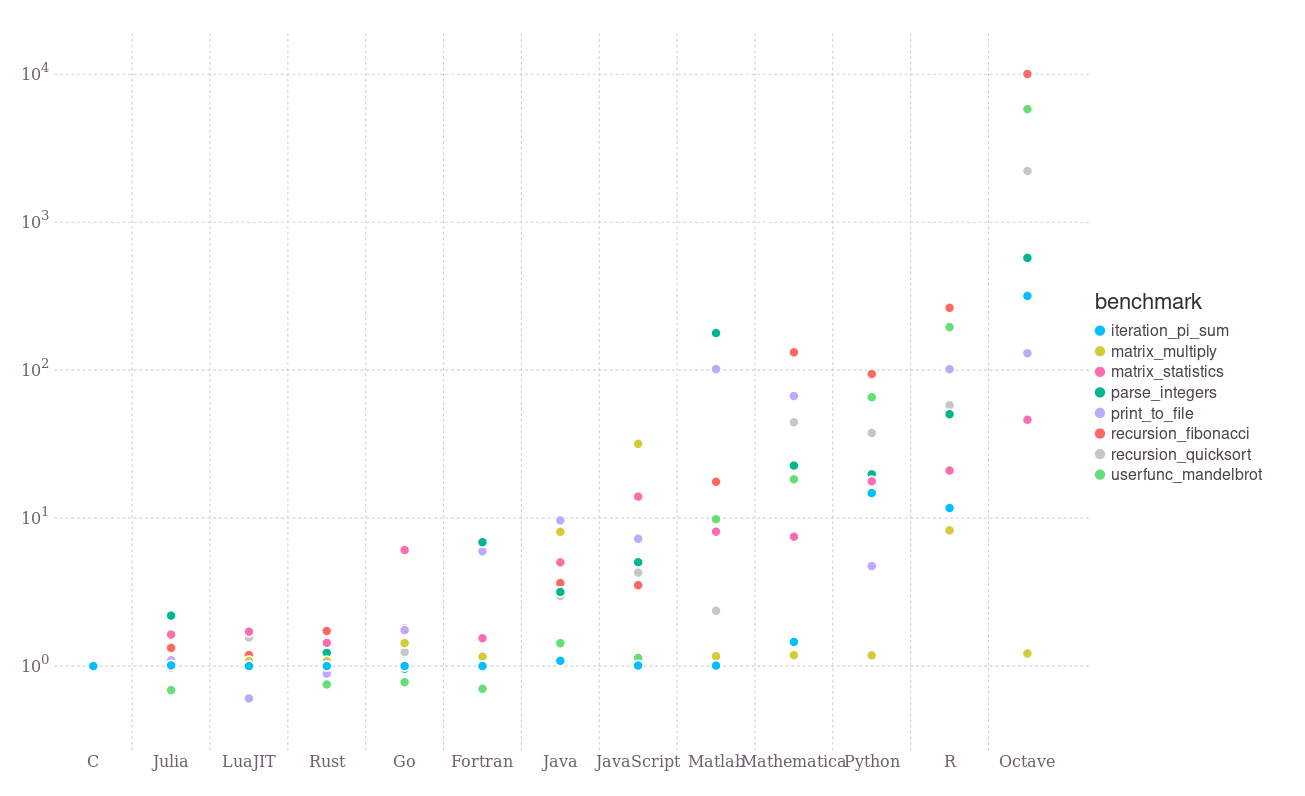
\includegraphics[width=.8\linewidth]{./figs/bench.png}
\end{center}
Micro-benchmarks from \url{https://julialang.org/benchmarks/}
\end{frame}

\begin{frame}[label={sec:orgacedcb7}]{The good: fast}
  \footnotesize
Julia is as fast as C and Fortan, but more productive:

\begin{center}
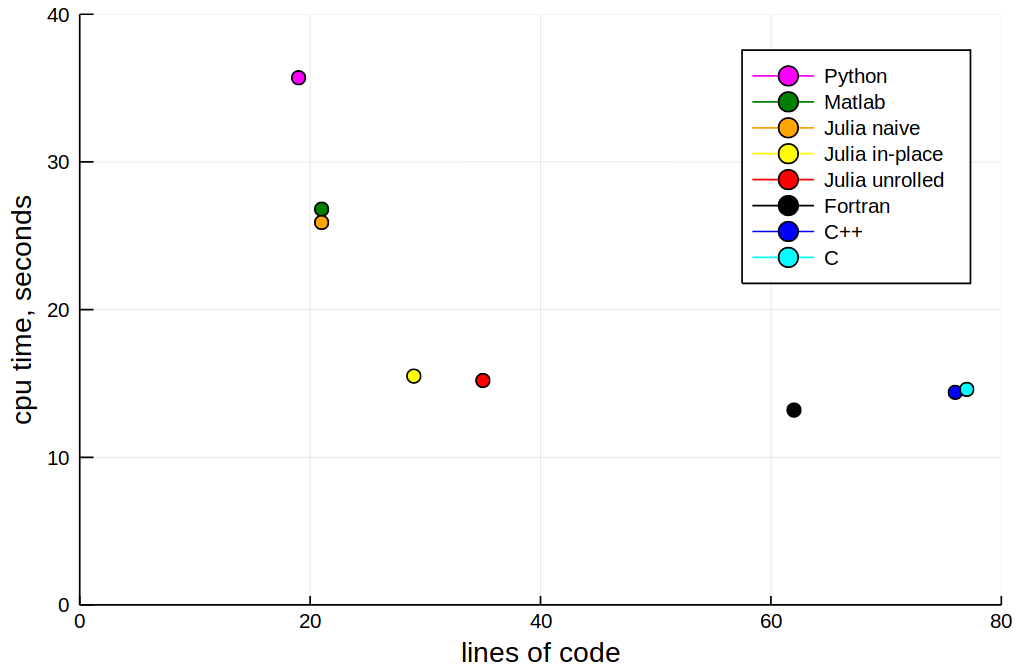
\includegraphics[width=.75\linewidth]{./figs/loc-vs-speed.png}
\end{center}

(c) \href{https://github.com/johnfgibson/julia-pde-benchmark/blob/master/1-Kuramoto-Sivashinksy-benchmark.ipynb}{@johnfgibson} solving the Kuramoto-Sivashinksy PDE (time + 1D space)
\end{frame}

\begin{frame}[label={sec:org7fa5452}]{Case-study: Celeste.jl}
  \footnotesize
Project to produce an accurate catalogue of 188 million astronomical objects

Ran on Cori supercomputer (@ Berkeley Lab):
\begin{itemize}
\item 1.54 petaflops using 1.3 million threads on 9,300 Knight Landing (KNL) nodes\\
--> the first dynamical language to \alert{join the petascale club}!
\item it took 15min to catalogue the objects using Bayesian techniques
\end{itemize}


\begin{center}
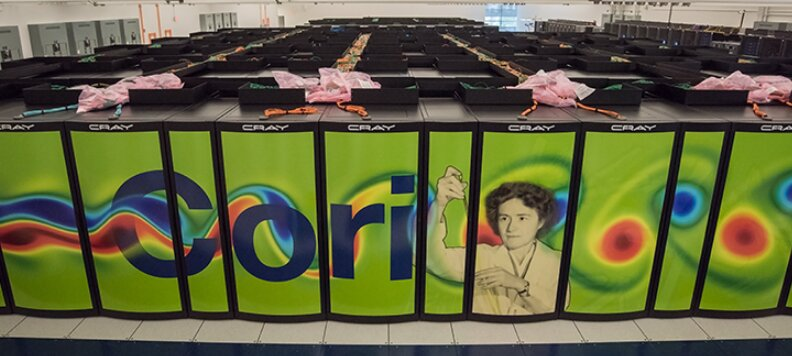
\includegraphics[width=.9\linewidth]{./figs/cori.jpg}
\end{center}
\end{frame}


\begin{frame}[label={sec:orga2001c6}]{Case-study: BITE-model}
  \footnotesize
The Bayesian Ice Thickness Estimation (BITE) model is a project of mine:
\begin{itemize}
\item simple forward model to calculate ice thickness maps
\item using Bayesian techniques (MCMC) to fit it to observations
\item fitted to 30'000 glaciers, calculated $10^8$ ice-thickness maps
--> Julia's performance needed
\end{itemize}

\begin{center}
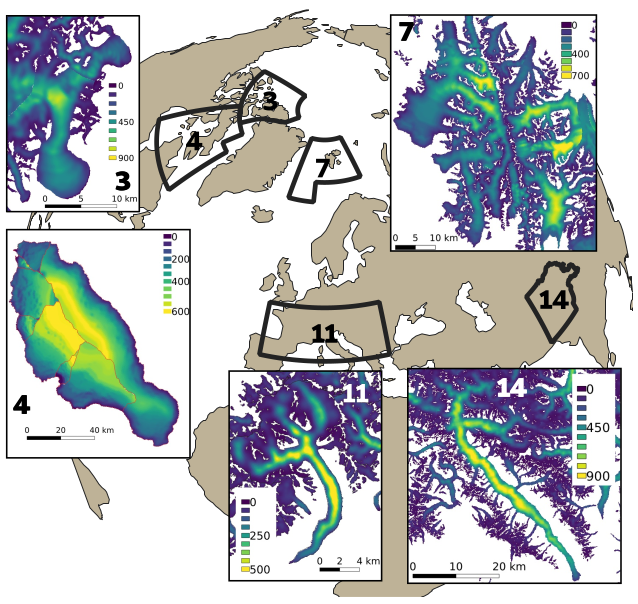
\includegraphics[width=.4\linewidth]{./figs/bite.png}
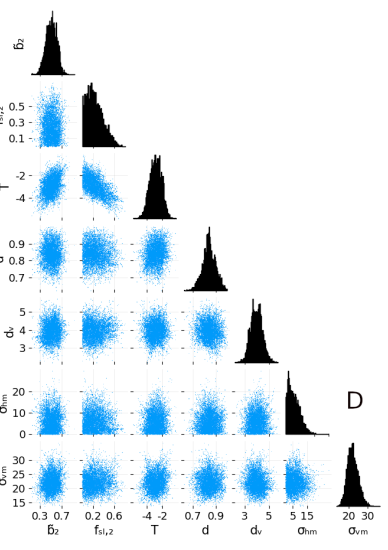
\includegraphics[width=.25\linewidth]{./figs/bite-2.png}
\end{center}
(Werder et al., 2020) \url{https://github.com/mauro3/BITEmodel.jl}
\end{frame}

\begin{frame}[label={sec:org5eae3db}]{Case-study: Julia at CSCS}
  \footnotesize
\alert{3D multi physics flow solver} in Julia running on Piz Daint
by Ludovic Räss (WSL/VAW Glaciology), Samuel Omlin (CSCS) \& Yury
Podladchikov (Uni Lausanne) (\href{https://ptsolvers.github.io/}{link})

\begin{itemize}
\item original code was a Matlab prototype + CUDA C + MPI production code
\item Julia code running on 5120 NVIDIA Tesla P100 GPUs on the hybrid Cray XC-50
showing nearly perfect scaling
\end{itemize}

\begin{center}
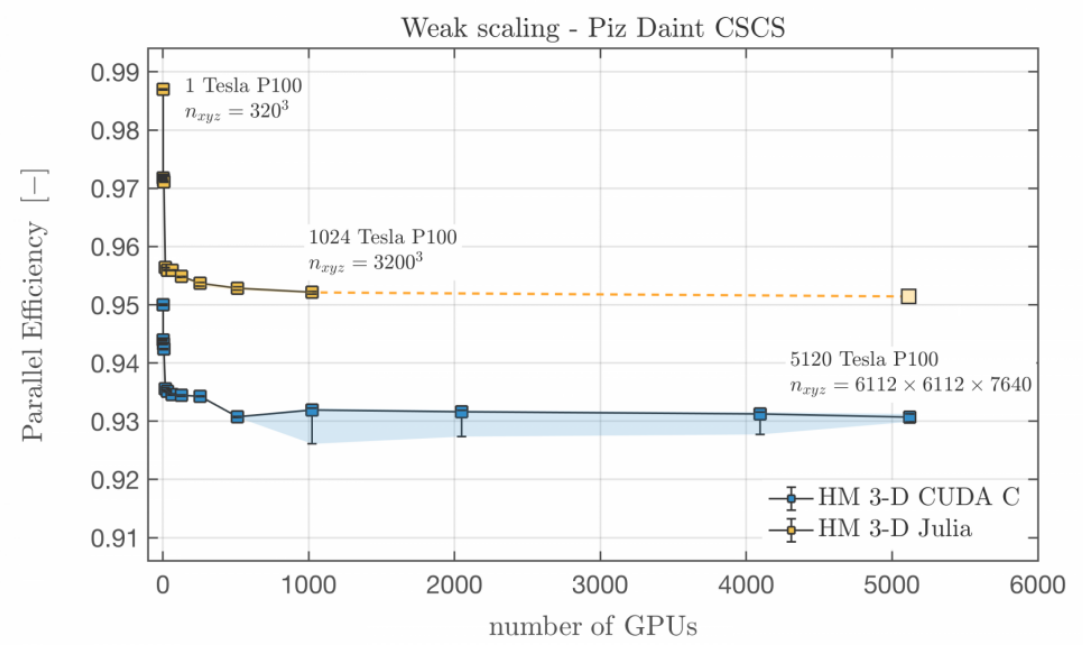
\includegraphics[width=.7\linewidth]{./figs/piz-daint.png}
\end{center}
\end{frame}

\begin{frame}[label={sec:org2946c39}]{The good: cutting-edge}
  \footnotesize
Whilst the breath of the package ecosystem is not comparable to, say,
Python.  There are many \alert{cutting-edge} packages (see this afternoon).

% \begin{itemize}
% \item \href{https://github.com/JuliaDiffEq/DifferentialEquations.jl}{DifferentialEquations.jl}, probably the best differential equation
% solver package around
% \item \href{https://fluxml.ai/2019/02/07/what-is-differentiable-programming.html}{Flux.jl} machine learning/differentiable programming package
% \item \href{https://github.com/JuliaOpt/JuMP.jl}{JuMP.jl} mathematical optimisation package, big in, e.g., operations
% research
% \item automatic differentiation (AD).
% \begin{itemize}
% \item \href{https://github.com/JuliaDiff/ForwardDiff.jl}{ForwardDiff.jl} \& \href{https://github.com/JuliaDiff/ReverseDiff.jl}{ReverseDiff.jl} (operator overloading)
% \item \href{https://github.com/FluxML/Zygote.jl}{Zygote.jl} (source transformation)
% \end{itemize}

% --> above packages can work together to allow \emph{Scientific machine
%     learning}, combining complex physical models with machine learning:
%     \url{https://fluxml.ai/blog/2019/03/05/dp-vs-rl.html}

% \item etc.
% \end{itemize}
\end{frame}

\begin{frame}[label={sec:orgebef73a}]{The good: community}
  \footnotesize
Last, the Julia community is very friendly and helpful:

\begin{itemize}
\item Easy to get help on the \href{https://discourse.julialang.org}{discourse forum}, StackOverflow and on \href{https://julialang.slack.com/}{Slack}
\item Active developer community on GitHub
\item \href{https://juliacon.org}{JuliaCon} is as fun and friendly (next one in July fully online and at MIT)
\end{itemize}

\end{frame}

% \begin{frame}[label={sec:org884d36c}]{The good: fun to program}
%   \footnotesize
% {\bf I really like programming in Julia!}\\
% I prefer it to: Python, Fortran, Matlab\ldots{}


% \end{frame}

\begin{frame}[label={sec:org87110ce}]{The bad}
  \footnotesize
\begin{itemize}
\item There are no interface-based abstractions in the language
\item It is not a statically compiled language and thus it does not have
the associated safety features.
--> there might be static checkers coming in the future
\end{itemize}
\end{frame}

\begin{frame}[label={sec:orgd4030d7}]{The ugly}
  \footnotesize
\begin{itemize}
\item \large Compilation times can be very long.  E.g. time to first plot can
20s+ (but fast afterwards)
\begin{itemize}
\item in general there are improvements from Julia version to version
  but it is still far from satisfying
\item apparently Julia 1.9, coming out in the next few weeks, should
  improve significantly on that again
\end{itemize}
\end{itemize}
\end{frame}



\begin{frame}[label={sec:orge9a7aab}]{Conclusions}
  \begin{center}

\includegraphics[width=.2\linewidth]{./figs/julia-logo.png}\quad 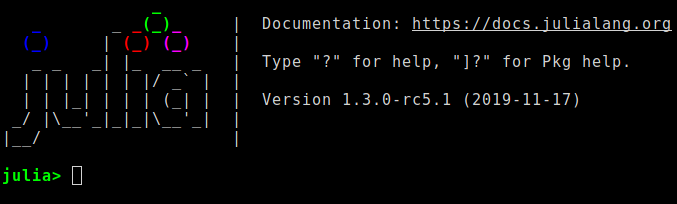
\includegraphics[width=.3\linewidth]{./figs/julia-repl.png}
\end{center}

  \footnotesize
\begin{itemize}
\item Julia sure is fast and fun
\item solves the two language problem \& blurs lines between devs and users
\end{itemize}
\vspace{5mm}
\pause

Let's get started then!

\end{frame}
\end{document}
%%% Local Variables:
%%% mode: latex
%%% TeX-master: t
%%% TeX-engine: xetex
%%% TeX-command-extra-options: "-shell-escape"
%%% End:
